\section{Server}

The demand for temporal isolation is undeniably becoming a main important discussed topics as the aim of this method of scheduling was to combine and merge not only all real-time tasks together, but also including the non-real-time tasks as well. Resource Reservation represents the most powerful technique of scheduling which is used to achieve such a desired property \cite{b1}. Therefore, it is certainly useful in preserving hard tasks from overruns that are caused by the soft tasks if we are dealing with a composed set of both soft and hard tasks at one time \cite{b4}. An essential property that must be ensured intending to run multiple concurrent tasks in computing system is temporal protection. This can prevent unexpected overruns that happens in a task from giving a bad impact on the execution of other tasks. In terms of hardware part, this is achieved by having each task or set of tasks assigning a fragment of the CPU and scheduling in a manner that it would acquire more bandwidth than it has been allotted. By using this approach, the capacity of processor is viewed as a finite resource that can be reserved, just as disk blocks and physical memory \cite{b2}.

As for the implementation of resource reservation, a real-time server, also known as reservation server, will be assigned to each of the application in a system. In a server, there must be a budget which denotes by the letter Q, period which denotes by the letter P and α which indicates the ratio of Q/P, and it is called the bandwidth of the server. Later, we will come across again with those terms stated before and also some equations related to them when we dive more into each type of servers’ insights. It is known that when we schedule soft aperiodic tasks and hard aperiodic tasks, we may encounter some issues while managing them under dynamic priority assignments \cite{b4}.

Therefore, several different service methods or servers have been introduced to solve these problems by implementing different approaches but with the same purpose which is to reduce the average response time of aperiodic requests without jeopardizing or make concessions on the schedulability of the existing hard periodic tasks in the system. Some of the popular dynamic servers proposed are Constant Bandwidth Server (CBS) alongside with other two predecessor algorithms which are the Total Bandwidth Server (TBS) and Earliest Deadline Late Server (EDL). We will be discussing on all three of algorithms stated because they are quite interconnected with each other, but we will only be emphasizing on CBS. In general, they are somehow quite similar to each other for the reason that all of the periodic tasks in the system will be scheduled or handled by using Earliest Deadline First (EDF) algorithm. Concerning the fixed-priority assignments, dynamic scheduling are characterized by higher schedulability bounds, since it can increase the size of aperiodic servers, enhance aperiodic responsiveness, thus making the processor to be better utilized \cite{b6}. 

\subsection{Total Bandwidth Server (TBS)}

Total Bandwidth Server or TBS uses an approach which enhancing the response time of an aperiodic task by assigning a possible short deadline to each of the aperiodic request. The assignment needs to be completed in the manner that the whole processor utilization of the aperiodic load would never go beyond the predefined maximum value which denotes by $U_{s}$. In other words, the server basically works as if each time an aperiodic task requesting to enter the system or if any aperiodic request is initiated to system, the total bandwidth of the server is immediately assigned to it whenever possible \cite{b6}.

As a matter of fact, TBS is one of the simplest servers to implement in dynamic priority server. This is due to the fact that it only needs to monitor the deadline which has been assigned to the last aperiodic request, so as to apply the appropriate deadline to the newly issued request. The request then can be sequenced into the ready queue and this is when the EDF will process it just like any other periodic task. Hence, the overhead is only due to the increased length of the ready queue if several aperiodic requests are pending concurrently. This problem can be overcome by organising a separate First In First Out (FIFO) queue for aperiodic requests, and inserting only the first one into the ready queue and so this extent, the overall overhead is practically negligible \cite{b2}.

\subsection{Earliest Deadline Late Server (EDL)}

We can see that just by implementing a simple design of algorithm, TBS still capable of achieving great response times for aperiodic tasks. Nevertheless, we could still acquire more fulfillment by improving some other important factors. EDL server is introduced to improve TBS server and the improvement of TBS that has been applied into EDL server is made by taking the advantage of the laxity or what we could say as leniency. As we know, as request arrives at the node of the system, the current executing periodic task have enough effective laxity, as in the interval between the completion time and the deadline to be safely preempted. Then, the idle times of an EDL scheduler are used to schedule aperiodic requests as soon as possible, postponing the execution of periodic tasks. Generally, when there are no aperiodic activities in the system, the periodic tasks are scheduled according to the EDF algorithm \cite{b8}.

As it has been pointed out, the EDL server schedulability’s synthesis is quite direct and straight. However, EDL server cannot be classified as a practical approach due to the complexity of computing the idle times at which each new aperiodic task arrives. This computation must be done each time considering whether the periodic task has been partially executed or maybe already done and completed when the aperiodic task arrive \cite{b8}.

\subsection{Constant Bandwidth Server (CBS) Insights}

Although the algorithms described in the previous sections are optimal, but they have too much overhead to be considered as a practical technique. Another TBS algorithm's key flaw is that it did not employ a server budget to manage the execution of aperiodic tasks. Instead, it only relies based on the information gained from the worst-case computation time enumerated by each task that arrives in the system. If those details are unavailable or unknown, which most likely happen because of highly variable execution times, then hard tasks are vulnerable of transient overruns that occurs in the soft tasks and will probably fail to meet their deadlines. Thus, in these instances, CBS algorithm may come in handy as it has an equivalent performance with TBS and it also has temporal isolation. 

In this section we will be exploiting the idea behind CBS server. This server uses a different strategy called the bandwidth reservation strategy and thus making it more efficient compared to other servers. It guarantees that, if $U_{s}$ is the fraction of processor time assigned to a server (namely its bandwidth), its contribution to the total utilization factor is no greater than $U_{s}$, even in the presence of overloads. This feature is unavailable in TBS implementation, whose actual contribution is limited to only $U_{s}$, in contingent of all the served jobs execute no more than the worst-case execution time that has been proclaimed.

The method used in CBS can be described briefly using an analogy of as new job enters the system, it is assigned to an appropriate scheduling deadline to make sure the demand does not exceed the allocated bandwidth. It is then enqueued in the ready queue of EDF. Whenever a task attempts to execute more than it is expected to execute, its deadline will be postponed and hence making its priority decreases. This is done to reduce the interference on the other tasks. Bear in mind that the task will still remain eligible for execution even though the deadline has been shifted back. This is why CBS is said to be a conserving algorithm because it basically accomplishes the available slack in an efficient way. Hence this will provide a better responsiveness not only towards non-work conserving algorithms but also towards other reservation approaches that schedule the extra portions of jobs in background \cite{b1}.

There will be no isolation between the tasks they are being managed by only a single server. This would also indicate that all the tasks in the subset will have to share the same bandwidth. In spite of that, other tasks outside the subset will be protected against overruns if such thing happens in the subset. That being the case, the server should be designed cautiously in terms of rules used for the deadline assignments to prevent any hard deadline to be missed when the system runs. 

Just like what has been mentioned in the system server earlier in paper, CBS has quite the same basic concept, but we use different annotations or letters to denotes the budget and the period of the server. In CBS, server budget is denoted by $c_{s}$ whereas the maximum budget and period of the server are denoted by $Q_{s}$ and $T_{s}$ respectively. The bandwidth of the server, $U_{s}$ is the ratio between $Q_{s}$ and $T_{s}$. As an additional detail, a fixed deadline $d_{s,k}$ is included in the server in which the dynamic deadline $d_{i,j}$ will be equal $d_{s,k}$, whenever a job $J_{i,j}$ is served. Concurrently, the value of $c_{s}$ will be decreases each time it is used when there exist a served job taking into account that the value of $c_{s}$ must be greater than zero. If the server budget, $c_{s}$ is finished or empty, it will be recharged at its maximum value $Q_{s}$ and a new server deadline will be created as $d_{s,k}+1 = d_{s,k} + T_{s}$  \cite{b2}. 

If there exist pending jobs, then a CBS is meant to be in an active state meanwhile when there are no pending jobs that need to be executed, then the state is in idle mode. Once a job $J_{i,j}$ arrives in which the server is active, the job request will be enqueued in a pending jobs queue in the manner of First In First Out (FIFO). In opposition to that, if a job $J_{i,j}$ arrives while server is in the idle state, we need to consider either the value of $c_{s}$ is greater than the value of $(d_{s,k} - r_{i,j})U_{s}$ or not. If it is greater, the server then generates a new deadline $d_{s,k}+1= r_{i,j} + T_{s}$, or else the job will be served with the last server deadline $d_{s,k}$ using the balance of the current budget $c_{s}$ and deadline. For a clearer view upon this algorithm, an example of a scenario with a diagram is provided below to help in understanding the process step by step \cite{b2}.

\begin{figure}[htp]
    \centering
    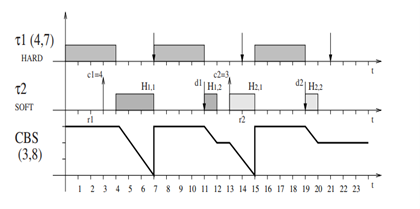
\includegraphics[width=7.5cm]{cbs}
    \caption{CBS implementation \cite{b2}.}
    \label{cbs}
\end{figure}

From ``Fig.~\ref{cbs}'' , we can see that the tasks are divided into two which are hard periodic task which denotes by $\tau_{1}$, and soft task scheduled together which denotes by $\tau_{2}$. Both tasks are served by a CBS with a maximum budget,  $Q_{s}$ of 3 and period, $T_{s}$ of 8. Hard periodic task, $\tau_{1}$ is set with a computation time, $c_1$ of 4 and period,  $T_{1}$ is equal to 4. The first job for the soft task, $\tau_{2} (J_{2,1})$ is initiated at (r1) = 3 while the server is inactive state, and it requires 4 units time of execution. Since $c_{s} \geq (d_{0}-r_{1})U_{s}$, the job is assigned a deadline $d_{1} = r_{1} + T_{s} = 11 $ and $c_{s}$ is recharged till in reaches the maximum budget which is 3. Since the budget, $c_{s}$ is being fully utilised at time t = 7, it will later be recharged again. Therefore, the server will generate a new deadline, $d_{2} = d_{1}+Ts$, thus making the new deadline, $d_{2} = 19$. Since the server deadline is postponed, $\tau_{1}$ will be executed until it completes as it emerges as the task with the earliest deadline \cite{b2}.

Subsequently, $\tau{2}$ is now resumed and the first job that is being postponed before is completed at time t = 12, and making the budget left equal to 2. The second job of task $(\tau_{2}$ arrives at time $r_{2}) = 13$ and imposes execution time of 3 units. Since $c_{s}$ is smaller than $d_{2} − r_{2})Us$, then it is possible for the last server deadline $d_{2}$ to handle job $(J_{2,1}$. However, the server budget is drained at t = 15, hence a new server deadline, $d_{3}$ is generated making the deadline being shifted backwards to t = 27 which calculated using the previous formula $d_{3} = (d_{2}+T_{s})$. Not to forget the server budget, $c_{s}$ is once again being recharged until it achieves the maximum value which is 3. One more time, $\tau_{1}$ becomes the highest priority task and executes until time t = 19. As job (J1,3) finally completed, $\tau_{2}$ is now able to execute the task to complete job $(J_{2,1}$ at time t = 20. This means that the server budget is left to be 2 \cite{b2}.

\subsection{Constant Bandwidth Server Properties}

As we can observe so far, methods introduced in CBS provide a lot of useful qualities properties. The mechanism used is appropriate and convenient in assisting applications that includes complex computation. One of the most critical properties is the isolation property. This property can rigorously be expressed according to the theorem and lemma stated below. 

Theorem:
The CPU utilization of a CBS S with parameters $(Q_{s}, T_{s})$ is $U_{s} = Q_{s}/T_{s}$, independently from the computation times and the arrival pattern of the served jobs \cite{b2}.

Lemma:
Given a set of n periodic hard tasks with processor utilization Up and a set of m CBSs with processor utilization, the whole set is schedulable by EDF if and only if Up + Us ≤ 1 \cite{b2}.

Due to the general isolation property, we can utilize a bandwidth reservation approach to devote a portion of the CPU time to soft tasks which have long computation times. The most important implication of this discovery is that soft tasks can be scheduled alongside hard tasks without compromising the priori guarantee, even if the soft task execution timings are unknown or the soft requests exceed the predicted load. Any time saved due to early completions is automatically reclaimed by CBS. This is because, if the budget is depleted, it is always refilled at its maximum value and the deadline of the server will be postponed. As a result, the server retains its eligibility, and the server budget can be used for the pending requests with the current deadline \cite{b2}. 

\subsection{Simulation Results Comparing TBS and CBS}

Next, we come to the simulation result when comparing TBS and CBS to reassure the findings that we have learned so far from this paper. Since we stated that CBS brings improvement and have better performance than TBS, thus in this segment, we will see the whether the CBS is efficient enough to handle the soft aperiodic request. In our study, we discovered that CBS service technique enhanced the responsiveness by quite a large ratio when compared to TBS.

Basically, the test that is being run is comparing the mean tardiness undergo by the soft tasks as CBS and TBS are handling and managing them. The periodic tasks utilization factor which denotes by (UHard) is set to 0.6 in this experiment. Based on the graph below, we can see that CBS surpasses TBS in handling the tasks which has high variance of execution times. From the results given in ``Fig.~\ref{result}'', due to the worst-case supposition, TBS may cause the processor to be underutilised \cite{b2}.

\begin{figure}[htp]
    \centering
    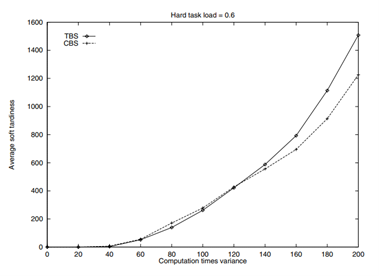
\includegraphics[width=7.5cm]{Picture3}
    \caption{Result on comparing TBS with CBS \cite{b2}.}
    \label{result}
\end{figure}

\subsection{Simulation Results Comparing TBS and CBS}

Next, a simple implementation of CBS can be simulated using a software called UPPAAL and in this section we will see the basic steps of methods used in CBS service mechanism. The steps can be divided into four different states. It is important to note that the simulation only covers the basic idea of CBS and not touching into the critical parts. 

\begin{figure}[htp]
    \centering
    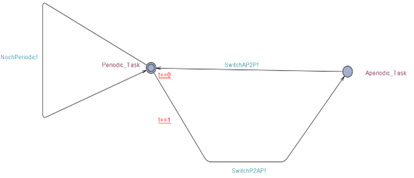
\includegraphics[width=7.5cm]{Picture4}
    \caption{Switching task processing \cite{b10}.}
    \label{ikan1}
\end{figure}

\begin{figure}[htp]
    \centering
    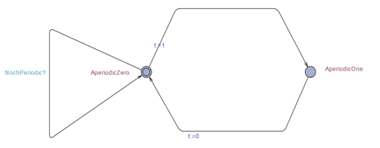
\includegraphics[width=7.5cm]{Picture5}
    \caption{Aperiodic is being handled \cite{b10}.}
    \label{ikan2}
\end{figure}

Based on ``Fig.~\ref{ikan1}'' and ``Fig.~\ref{ikan2}'', we can observe that the periodic task will always be chosen to be the executed if there is no request initiated by the aperiodic task to be executed. If there is no request from the aperiodic task, it will merely loop into the periodic task, as shown in the diagram. In order to switch from executing periodic task to executing aperiodic task, the mode must be changed from idle to active. The CBS mode on the other hand, must first identify whether the server budget is available or not in order to execute the aperiodic task. Theoretically, CBS will only be in active state if there exist a pending jobs. This will be explained by using the figures below.

\begin{figure}[htp]
    \centering
    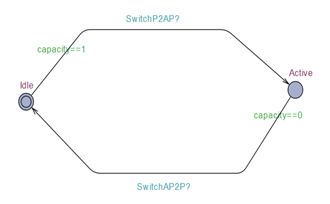
\includegraphics[width=7.5cm]{Picture6}
    \caption{CBS mode changes \cite{b10}.}
    \label{bulat1}
\end{figure}

\begin{figure}[htp]
    \centering
    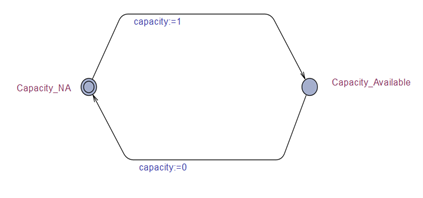
\includegraphics[width=7.5cm]{Picture7}
    \caption{State changes of CBS server budget (capacity) \cite{b10}.}
    \label{bulat2}
\end{figure}


In ``Fig.~\ref{bulat1}'' and ``Fig.~\ref{bulat2}'', the state and mode changes of CBS are shown to indicate that CBS mode may change if the server capacity or server budget is available which denoted by (capacity = = 1). It will then switch again to the idle state if the server budget is exhausted or already fully being utilized by the served tasks which denotes by (capacity = = 0). To run this simulation, a GitHub link is provided on the reference section.